% =============================================================================
% Policy Note: Climate Change Risk Scenarios and Mitigation for Lao PDR
% OECD Development Center
% =============================================================================
\documentclass[11pt,a4paper]{article}

% --- Packages ---
\usepackage[margin=2.5cm]{geometry}
\usepackage{graphicx}
\usepackage{float}
\usepackage{booktabs}
\usepackage{hyperref}
\usepackage{xcolor}
\usepackage{titlesec}
\usepackage{caption}
\usepackage{parskip}
\usepackage{enumitem}
\usepackage{array}
\usepackage{multirow}
\usepackage{setspace}
\usepackage{amsmath,amssymb}
\onehalfspacing

% --- OECD colors ---
\definecolor{oecdblue}{HTML}{002F6C}
\definecolor{oecdlightblue}{HTML}{006BB6}

% --- Section formatting ---
\titleformat{\section}
  {\Large\bfseries\color{oecdblue}}{\thesection}{1em}{}
\titleformat{\subsection}
  {\large\bfseries\color{oecdlightblue}}{\thesubsection}{1em}{}

% --- Hyperref setup ---
\hypersetup{
  colorlinks=true,
  linkcolor=oecdblue,
  citecolor=oecdblue,
  urlcolor=oecdlightblue
}

% --- Caption styling ---
\captionsetup{font=small, labelfont=bf}

\begin{document}

% =============================================================================
% TITLE
% =============================================================================
\begin{center}
  {\LARGE\bfseries\color{oecdblue} Climate Change Risk Scenarios\\[4pt]
  and Mitigation Strategies for Lao PDR}\\[12pt]
  {\large\textbf{OECD Development Center, Resilient and Sustainable Development Strategies}}\\[8pt]
  {\normalsize Camilo Saldarriaga \quad Jesse Grabowski \quad Jan Rielaender}\\[4pt]
  {\small March 2026}
\end{center}

\vspace{1em}
\noindent\rule{\textwidth}{0.5pt}
\vspace{0.5em}

\noindent\fcolorbox{oecdblue}{white}{%
\begin{minipage}{0.96\textwidth}
\vspace{0.5em}
\textbf{\color{oecdblue} Abstract}\\[6pt]
{\small\itshape
This policy note applies the Probabilistic Geospatial Risk (PGR) model---a fully Bayesian framework integrating disaster frequency, damage severity, geospatial patterns, and climate projections---to quantify Lao PDR's exposure to climate change-related disasters. Baseline projections show that disaster frequency is expected to double by 2055, with return period damages rising substantially. To understand how different global CO\textsubscript{2} trends affect this exposure, we apply a scenario analysis using five IPCC Shared Socioeconomic Pathways (SSP) CO\textsubscript{2} concentration trajectories (SSP1-19 through SSP5-85). Crucially, we do not vary CO\textsubscript{2} in isolation: using the innovation covariance learned by our multivariate Bayesian time series model, we propagate each CO\textsubscript{2} scenario to conditionally adjust ocean temperature and precipitation covariates. The analysis reveals that higher emissions translate into substantially greater disaster risk, with the gap between scenarios widening dramatically over time. Under the most pessimistic pathway (SSP5-85), 100-year return period damages reach USD~4.6 billion by 2055. Critically, the most optimistic pathway (SSP1-19) not only slows the increase but actually reverses the damage trend after the mid-2040s, demonstrating that ambitious mitigation can bend the disaster risk curve downward. Flood wall simulations demonstrate that targeted infrastructure can reduce damages by up to 73\% in cities where river proximity dominates the risk profile, but yield minimal benefit where other factors drive exposure. These results underscore the need for evidence-based, location-specific adaptation investments informed by probabilistic risk decomposition, alongside ambitious global emission reductions.
}
\vspace{0.5em}
\end{minipage}}

\newpage

% =============================================================================
% 1. INTRODUCTION
% =============================================================================
\section{Introduction}

This policy note presents scenario-based extensions of the Probabilistic Geospatial Risk (PGR) model developed to quantify Lao PDR's exposure to climate change-related disasters. The methodology, detailed in the methodological paper \textit{``Estimating Climate Change Risk Exposure: A Probabilistic Approach''} \cite{saldarriaga2026}, integrates multiple statistical models to estimate disaster frequency, damage severity, and geospatial risk patterns using a fully Bayesian framework.

Lao PDR is a landlocked country in Southeast Asia with a population of approximately 7.5 million and a GDP of roughly USD~20 billion. The country is highly exposed to hydrometeorological hazards due to its geography: the Mekong River and its tributaries traverse the entire territory, and annual monsoon seasons bring intense and prolonged rainfall. Historical disasters have caused significant economic damage---most notably, the 2018 collapse of the Xe-Pian Xe-Namnoy dam displaced thousands and caused hundreds of millions of dollars in damages \cite{emdat2024, laopdr_pdna2018}. Despite this high exposure, Lao has limited fiscal capacity to absorb disaster shocks: public debt already exceeds 100\% of GDP, and the country relies heavily on external assistance for post-disaster recovery. This combination of high hazard exposure and low absorptive capacity makes proactive risk assessment and targeted adaptation investments particularly critical for Lao PDR \cite{ipcc2022ar6wg2}.

The PGR model focuses on hydrometeorological disasters---storms, floods, and movements of wet masses---which represent more than 50\% of the disasters reported in Lao during the last decades and have a direct link with climate change \cite{lopez2015, vanaalst2006}. The approach uses Bayesian statistics, which enables a robust measurement of uncertainty and allows us to consider not just the mean values of possible events but also to understand how extreme events can affect the country by estimating the entire probability distributions.

Existing approaches to disaster risk assessment in developing countries often rely on deterministic models or historical averages, which fail to capture extreme tail events that pose the greatest threat to economic stability \cite{cavallo2011, howard2017}. The PGR model addresses these limitations by producing full probability distributions of damages, enabling policymakers to assess not only expected costs but also the probability of worst-case outcomes that could overwhelm national response capacity.

This note first presents the baseline results of the PGR model for Lao PDR, and then addresses two policy-relevant questions:

\begin{enumerate}[leftmargin=2em]
  \item \textbf{What are the baseline projections for Lao's climate risk?} We present the model's estimates of how disaster frequency, severity, and geospatial patterns are expected to evolve under current trends.

  \item \textbf{How do different CO\textsubscript{2} emission scenarios affect Lao's exposure to climate change risk?} We feed five IPCC Shared Socioeconomic Pathways (SSP) CO\textsubscript{2} concentration trajectories into the model---adjusting all correlated climate covariates accordingly---to compare how alternative global emission pathways translate into different levels of disaster risk for Lao PDR.

  \item \textbf{How can local infrastructure interventions mitigate disaster risk in specific cities?} We simulate the construction of flood walls in three Laotian cities by modifying the geospatial model's distance-to-river variable, and evaluate the resulting reduction in expected damages.
\end{enumerate}

The analysis concludes that Lao PDR faces substantially increasing risks under baseline projections, with return period damages rising sharply over the coming decades. Under higher emission scenarios (SSP3-70, SSP5-85), damages from extreme events could potentially double by 2055 relative to more optimistic pathways. Crucially, we show that global CO\textsubscript{2} pathways do matter in both directions: under the most optimistic scenarios (SSP1-19, SSP1-26), projected disaster frequency and damages not only grow more slowly but actually begin to decrease after the mid-2040s, demonstrating that ambitious mitigation can reverse---not merely slow---the escalation of climate risk. At the local level, flood wall interventions can achieve significant damage reductions in cities where proximity to rivers is the dominant risk factor.

% =============================================================================
% 2. MODELING APPROACH
% =============================================================================
\section{Modeling Approach}

\subsection{The PGR Model Pipeline}

The Probabilistic Geospatial Risk (PGR) model is a seven-component Bayesian system designed to quantify climate change risk exposure at both national and local levels. The methodology focuses on natural disasters as a key channel through which climate change affects the economy: climate researchers widely agree that disasters will become more frequent and severe with climate change \cite{ipcc2023ar6, nordhaus2019}, the quantification of damages from discrete disaster events is tractable, and specific actionable recommendations can be made to policymakers based on the results.

The model uses a Bayesian probabilistic approach, implemented in the PyMC framework \cite{abril2023pymc}, which provides three crucial advantages over traditional statistical methods. First, Bayesian inference allows the use of flexible probability distributions---such as zero-inflated and heavy-tailed models---that better capture the empirical patterns of disaster data. Second, it estimates entire probability distributions rather than point estimates, enabling the study of distribution tails where the most impactful events occur. Third, uncertainty is propagated from intermediate estimates (disaster frequencies, economic vulnerabilities) into the final risk exposure outputs, ensuring that the results reflect both data limitations and model uncertainty.

Figure~\ref{fig:pgr_diagram} presents the seven-component architecture of the PGR model. The components are described below.

\begin{figure}[H]
  \centering
  
\includegraphics[width=\textwidth]{images/modeling_approach.png}
  \caption{Architecture of the Probabilistic Geospatial Risk (PGR) model. Seven interconnected components combine disaster frequency, damage severity, geospatial patterns, and climate projections to produce geolocalized damage curves. Adapted from \cite{saldarriaga2026}.}
  \label{fig:pgr_diagram}
\end{figure}

\begin{enumerate}[leftmargin=2em]
  \item \textbf{Disaster frequency model.} This component estimates the probability distribution of the number of hydrometeorological disasters a country experiences per year. The model uses a Zero-Inflated Negative Binomial distribution, which captures two empirical features of the data: many country-years have zero reported disasters (the zero-inflation component), and the variance of disaster counts exceeds the mean (the negative binomial component). The model is estimated as a hierarchical Bayesian panel regression across countries and years, with country-level fixed effects, spatial random effects using the Besag--York--Molli\'{e} (BYM) specification \cite{besag1991}, and covariates including atmospheric CO\textsubscript{2}, precipitation deviation, GDP per capita, and population density. The hierarchical framework enables partial pooling of information across countries, improving estimates for data-sparse countries like Lao PDR.

  \item \textbf{Disaster damage model.} This component estimates the expected monetary cost of each disaster, conditional on its occurrence. It uses a Hurdle LogNormal distribution, which separates the process into two parts: a binary model for whether a disaster causes any reported damage, and a truncated LogNormal model for the magnitude of positive damages. This specification is well-suited to disaster cost data, which exhibits both a mass of zero-damage events and a heavy right tail---rare extreme events can generate damages orders of magnitude larger than the median \cite{cavallo2011, howard2017}. The covariate structure mirrors that of the frequency model, with the same hierarchical country effects allowing the model to learn country-specific relationships between economic development and disaster severity.

  \item \textbf{Geospatial risk model.} This component models the probability of a disaster occurring at each specific point within a country. It uses a Hilbert Space Gaussian Process (HSGP) \cite{solin2020}, a computationally efficient approximation to a full Gaussian Process that makes it feasible to estimate spatial patterns over tens of thousands of grid points. The HSGP learns smooth spatial surfaces from historical disaster coordinates using a Mat\'{e}rn 5/2 kernel, effectively identifying which areas are more disaster-prone based purely on the geography of past events. In the full model, these learned spatial patterns are combined with measurable geographic features---specifically, the logarithmic distance to the nearest river \cite{lehner2013} and the logarithmic distance to the coastline---as well as country-level climate and economic covariates. The model is estimated at the regional scale (Lao PDR and its neighboring countries), using a binary classification framework that distinguishes observed disaster locations from synthetic non-disaster points generated across the country's map.

  \item \textbf{Time series forecasting.} To project the models into the future, the PGR system estimates Bayesian Exponential Time Smoothing (ETS) state-space models for each covariate. These models project country-level variables (real GDP, population, precipitation) and global climate indicators (atmospheric CO\textsubscript{2}, ocean temperature deviation) forward in time. Besides modeling the long term trend of the different covariates, we also model how ocean temperature and precipitaion evolve conditional on the atmospheric CO2 trajectory given by each IPCC scenario. For this we take advantage of teh covariance structure obtained by modeling jointly all the variables.

  \item \textbf{Country-level damage curves.} The frequency and damage models are combined to produce the full probability distribution of annual disaster damages. By multiplying the estimated number of events by the expected damage per event across all posterior draws, the model generates a joint distribution that captures both the probability of disasters occurring and their potential severity. The key output is expressed in terms of \textit{return years}: a 100-year return period (100-RY) event corresponds to the damage level that has a 1\% chance of being exceeded in any given year---or equivalently, the damage level one would expect to be equaled or exceeded once every 100 years on average. Frequent events (low return years) are more common but cause less damage; rare events (high return years) are less frequent but can cause devastating damage when they occur. The Bayesian approach is particularly valuable here because disaster damage distributions are typically heavy-tailed: the mean is not a good summary of the risk, and it is precisely the tail behavior---captured by high return-year quantiles---that is most policy-relevant.

  \item \textbf{Geolocalized damage curves.} The country-level damage curves are spatially disaggregated using the geospatial model's probability surface. Each location receives a share of the national expected damages proportional to its estimated disaster probability. This produces location-specific damage curves that account for the geographic heterogeneity of risk within the country, enabling the identification of the most vulnerable areas and the prioritization of local adaptation investments.

  \item \textbf{Future exposure assessment.} All components are integrated with the time series projections to assess how risk evolves over time. As atmospheric CO\textsubscript{2} increases, ocean temperatures rise, and population grows, the model projects how disaster frequency, severity, and spatial distribution shift---producing forward-looking damage curves that quantify the escalating cost of climate inaction.
\end{enumerate}

\subsection{CO\textsubscript{2} Scenario Analysis}

A central application of the PGR model is evaluating how alternative global emission pathways affect Lao PDR's disaster risk. The IPCC's Sixth Assessment Report (AR6) \cite{ipcc2023ar6} uses Shared Socioeconomic Pathways (SSPs) to describe plausible futures for global CO\textsubscript{2} concentrations under different socioeconomic and policy assumptions. We use five scenarios that span the full range of possibilities, described in Table~\ref{tab:ipcc_scenarios}. The atmospheric CO\textsubscript{2} concentration data for each scenario comes from the Reduced Complexity Model Intercomparison Project (RCMIP) \cite{nicholls2021rcmip}. Notably, current global emissions trajectories are heading between SSP2-45 and SSP3-70 under existing policies \cite{ipcc2021ar6wg1}.

\begin{table}[H]
  \centering
  \caption{IPCC SSP CO\textsubscript{2} concentration scenarios used in the analysis.}
  \label{tab:ipcc_scenarios}
  \small
  \begin{tabular}{llp{9cm}}
    \toprule
    \textbf{Scenario} & \textbf{Level} & \textbf{Key Assumptions} \\
    \midrule
    SSP1-19 & Very low  & Sustainability-focused development with rapid decarbonization. Net-zero CO\textsubscript{2} emissions around 2050, net-negative thereafter. Limits warming to 1.5\textdegree C. The most ambitious pathway, requiring immediate and large-scale emission reductions. \\[4pt]
    SSP1-26 & Low       & Strong sustainability policies with robust mitigation efforts. Limits warming to approximately 2\textdegree C by 2100. Represents a world that achieves the Paris Agreement targets. \\[4pt]
    SSP2-45 & Moderate  & Middle-of-the-road development with moderate mitigation. Social, economic, and technological trends broadly follow historical patterns. CO\textsubscript{2} concentrations stabilize by end of century. \\[4pt]
    SSP3-70 & High      & Limited international cooperation on climate. High population growth in developing regions, slow technological progress, and weak environmental policies lead to high emissions. \\[4pt]
    SSP5-85 & Very high & Fossil-fueled development with rapid economic growth driven by energy-intensive lifestyles. Represents the most carbon-intensive trajectory, with CO\textsubscript{2} concentrations exceeding 1{,}100~ppm by 2100. \\
    \bottomrule
  \end{tabular}
\end{table}

\subsubsection{Conditional covariate adjustment}

A key methodological choice in the scenario analysis is how to treat covariates other than CO\textsubscript{2}. A naive approach would substitute only the CO\textsubscript{2} trajectory while holding all other variables (ocean temperature, precipitation, GDP, population) at their baseline projections. However, this ignores the fact that higher atmospheric CO\textsubscript{2} concentrations are physically linked to warmer ocean temperatures and altered precipitation patterns. Failing to adjust these covariates would understate the true divergence between scenarios.

We address this using the \textbf{multivariate Gaussian conditional distribution} applied to the innovation covariance matrix estimated by our Bayesian ETS time series model (Component~4 of the PGR pipeline). This model jointly estimates all five covariates with a dense innovation covariance, capturing the empirical correlations between their unexpected changes. The conditional expectation of any variable $X_j$ given a specific CO\textsubscript{2} value is:
%
\begin{equation}
  \mathbb{E}[X_j \mid \text{CO}_2 = c] = \mu_j + \frac{\text{Cov}(X_j, \text{CO}_2)}{\text{Var}(\text{CO}_2)} \cdot (c - \mu_{\text{CO}_2})
\end{equation}
%
where $\mu_j$ and $\mu_{\text{CO}_2}$ are the baseline forecasts. The regression coefficient $\beta_j = \text{Cov}(X_j, \text{CO}_2) / \text{Var}(\text{CO}_2)$ is computed from the posterior mean of the innovation covariance. Figure~\ref{fig:corr_matrix} presents the estimated innovation correlation matrix across all five covariates.

\begin{figure}[H]
  \centering
  \includegraphics[width=0.55\textwidth]{images/innovation_correlation_matrix.png}
  \caption{Innovation correlation matrix (posterior mean) from the multivariate Bayesian ETS model. The strongest cross-variable correlation is between CO\textsubscript{2} and ocean temperature ($r = 0.47$), reflecting the physical mechanism by which greenhouse gases trap heat in the ocean. Precipitation shows a weak negative correlation with CO\textsubscript{2} ($r = -0.08$).}
  \label{fig:corr_matrix}
\end{figure}

The strongest channel is CO\textsubscript{2}~$\to$~ocean temperature ($r = 0.47$), reflecting the physical mechanism by which greenhouse gases trap heat. The CO\textsubscript{2}~$\to$~precipitation correlation is weak ($r = -0.08$), but the adjustment is still applied to maintain internal consistency across climate variables. GDP and population, by contrast, are kept at their baseline projections. Although the covariance matrix shows nonzero correlations between CO\textsubscript{2} and these variables ($r = -0.20$ for GDP, $r = -0.14$ for population), adjusting them would not be appropriate: the causal link from atmospheric CO\textsubscript{2} concentrations to national economic output and demographic trends operates through indirect, long-run channels---such as economic restructuring, agricultural productivity shifts, health impacts, and migration---that are not captured by the contemporaneous innovation correlations estimated by the model. Applying the mechanical conditional adjustment to GDP and population based on these weak statistical associations would introduce noise rather than meaningful signal into the projections.

\subsubsection{Scenario analysis procedure}

For each SSP scenario, we construct a complete set of covariate trajectories where CO\textsubscript{2}, ocean temperature deviation, and precipitation deviation are all adjusted conditional on the scenario's CO\textsubscript{2} pathway. These scenario-specific covariates are then fed into the pre-trained PGR model to generate posterior predictive samples of disaster frequency, damages, and damage curves. This design captures both the \textit{direct} effect of CO\textsubscript{2} on disaster risk and the \textit{indirect} effects transmitted through correlated climate variables. Figure~\ref{fig:co2_scenarios} presents the five CO\textsubscript{2} concentration trajectories used in the analysis.

\begin{figure}[H]
  \centering
  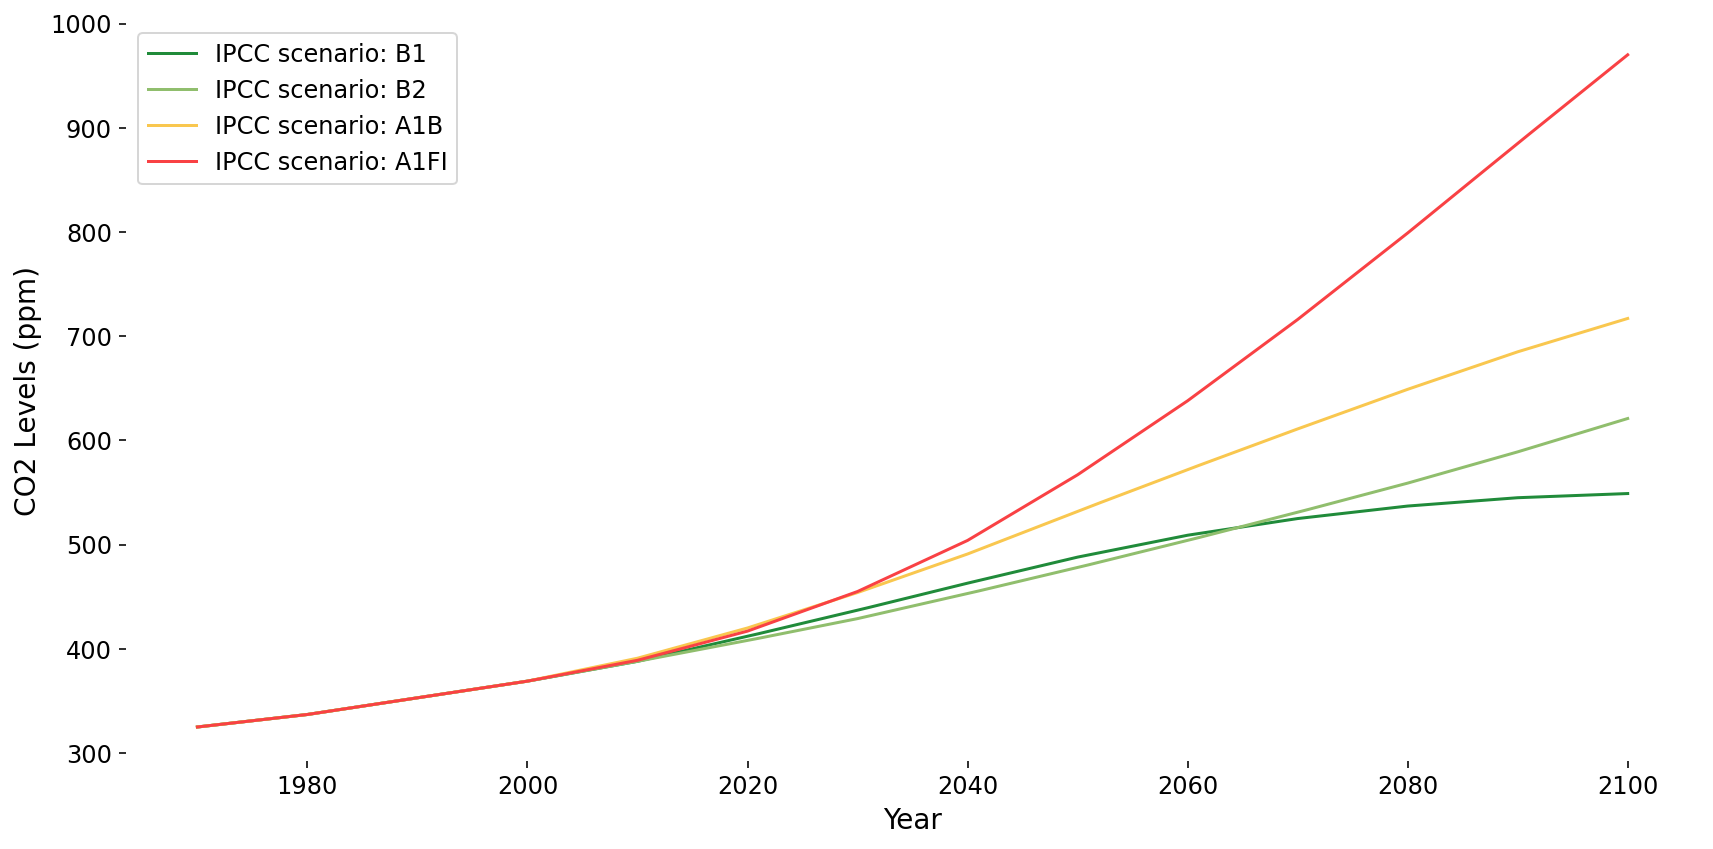
\includegraphics[width=0.95\textwidth]{../notebooks/policy_note/figures/ipcc_scenarios_co2.png}
  \caption{IPCC SSP atmospheric CO\textsubscript{2} concentration scenarios (SSP1-19 through SSP5-85) used as inputs to the PGR model. Data from the RCMIP dataset \cite{nicholls2021rcmip}. Higher scenarios correspond to more carbon-intensive development pathways.}
  \label{fig:co2_scenarios}
\end{figure}

\subsection{Flood Wall Simulations}

The second policy application of the PGR model evaluates the potential impact of local infrastructure interventions on disaster risk. The geospatial component of the model identifies the distance to the nearest river as a key driver of flood risk at specific locations. We exploit this relationship to simulate the effect of building flood walls in specific cities.

We cannot directly introduce a flood wall into the model, as it does not contain geospatial information regarding infrastructure. However, we can simulate its effect by making an equivalent change using the model's variables. The primary effect of a flood wall is to isolate a particular point from the flood risk posed by nearby water bodies. We achieve a similar effect by artificially increasing the value of the distance-to-river variable at the grid point corresponding to each city, effectively simulating the hydrological isolation that a physical flood wall would provide.

We define two intervention scenarios:

\begin{itemize}[leftmargin=2em]
  \item \textbf{Intermediate wall:} The distance-to-river is set to the \textit{median} value across the entire Laos prediction grid (approximately 48,000 grid points). This is equivalent to moving the city to a typical inland location, representing a moderate level of flood protection.
  \item \textbf{Full wall:} The distance-to-river is set to the \textit{maximum} value across the grid---equivalent to the most river-isolated point in Lao PDR. This represents the theoretical maximum benefit achievable through river isolation alone.
\end{itemize}

For each scenario, we recompute the full geospatial model predictions at the modified grid points and then generate new geolocalized damage curves for each city. The difference between the baseline and intervention damage curves measures the expected benefit of the flood wall in terms of reduced damages at various return periods. This methodology allows us to evaluate the current damage exposure of specific locations and to assess the potential economic returns of flood wall interventions based on expected damage reductions.

We apply these simulations to three cities: \textbf{Attapeu}, \textbf{Vientiane}, and \textbf{Pakse}, selected because they are population centers located near high-risk areas identified by the geospatial model.

It is important to note that this approach does not seek to replace detailed hydrological and topographical assessments. Rather, it provides a rapid, general, and cost-effective screening tool that can identify locations where more detailed engineering analysis is warranted.

% =============================================================================
% 3. DATA
% =============================================================================
\section{Data}

The PGR model draws on multiple data sources spanning disaster records, macroeconomic indicators, climate variables, and geospatial information. At the country level, disaster event counts and reported economic damages are obtained from the EM-DAT international disaster database \cite{emdat2024}. These are merged with World Bank Development Indicators---GDP per capita and population density \cite{worldbank_wdi_2024}---and with gridded precipitation data from the GPCC dataset \cite{gpcc_2022}, which is aggregated to country-level annual averages using national shapefiles. At the global level, two climate time series enter the model as covariates: atmospheric CO\textsubscript{2} concentration from NOAA's Mauna Loa observatory \cite{noaa_co2_2024} and ocean temperature deviation from the NOAA Global Surface Temperature Dataset \cite{zhang_noaa_2019}. For the geospatial component, we use World Bank country boundary shapefiles \cite{worldbank_wdi_2024} and the HydroRIVERS global river network dataset \cite{lehner2013}, from which we compute the distance from each point to the nearest river and coastline. The analysis focuses on hydrometeorological disasters (floods, storms, and wet mass movements) recorded after 1980 that affected more than 1,000 people, yielding 5,692 events worldwide. Full details on data processing are provided in the companion paper \cite{saldarriaga2026}.

\subsection{AI-Based Geolocation of Disaster Events}

A significant challenge for the geospatial component of the PGR model is the scarcity of geographic coordinates in disaster databases. Out of 5,692 hydrometeorological disasters in the EM-DAT database, only 864---approximately 15\%---have associated latitude and longitude coordinates. In contrast, 5,640 observations include a free-text ``Location'' field containing the names of affected places. This field is often complex: a single disaster may list multiple provinces, cities, and regions in inconsistent formats across different countries and languages.

To overcome this limitation, we developed an automated pipeline that sends each disaster's location text, along with its country and region, to OpenAI's GPT-4o-mini large language model \cite{openai2024gpt4omini}. The model is instructed to parse the text, identify individual locations, and return geographic coordinates for each one. A multi-stage validation process ensures data quality: the returned coordinates are spatially joined with country boundary shapefiles to verify that each point falls within the correct country, with a buffer applied to account for coastal and border imprecision. Points that fail this check are removed.

After processing, the pipeline transforms the textual location data into 2,876 individual coordinate points---more than tripling the original geospatial coverage of the database. Figure~\ref{fig:gpt_query} compares the spatial representation of disaster locations before and after the AI-based geocoding, showing the dramatic improvement in coverage. This enriched dataset is critical for training the HSGP geospatial model, which would otherwise be limited to the small fraction of events with pre-existing coordinates. The full methodology and validation results are detailed in \cite{saldarriaga2026}.

\begin{figure}[H]
  \centering
  
\includegraphics[width=0.85\textwidth]{images/gpt_query_comp.png}
  \caption{Disasters with geographic coordinates before and after the AI-based geocoding query. The left panel shows the 864 disasters with pre-existing coordinates in EM-DAT. The right panel shows the expanded set of 2,876 coordinate points after processing location text through GPT-4o-mini.}
  \label{fig:gpt_query}
\end{figure}

\subsection{Synthetic Non-Disaster Points for Model Training}

The geospatial component of the PGR model estimates the probability of a disaster occurring at each specific point within a country. To train this model, we need both positive examples (locations where disasters occurred) and negative examples (locations where they did not). We generate synthetic non-disaster points by randomly placing 15 points within the country boundaries for each real disaster location. This ratio was determined through extensive testing to produce high-quality posterior samples for the HSGP model.

The disaster and synthetic non-disaster points are merged into a single training dataset. For each point---whether real or synthetic---we compute the logarithmic distance to the nearest river and the nearest coastline, and assign the relevant country-level covariates for the corresponding year. All features are standardized before estimation. The geospatial model is trained at the regional scale: for Lao PDR, the training data includes disaster points from Cambodia, Thailand, Laos, and Vietnam. Figure~\ref{fig:synth_points} shows the spatial distribution of real disaster points and synthetic non-disaster points across the region.

It is important to note that the disaster-to-non-disaster ratio does not affect the final probability estimates, as the model outputs are normalized by dividing each point's probability by the sum across all points. The synthetic points serve only to provide the model with a representative sample of geographic locations against which to contrast the observed disaster patterns.

\begin{figure}[H]
  \centering
  
\includegraphics[width=0.5\textwidth]{images/laos_neigh_real_synth_dis.png}
  \caption{Disaster and synthetic non-disaster points for Cambodia, Thailand, Laos, and Vietnam. Yellow points correspond to geocoded disaster locations; purple points are randomly generated non-disaster locations used for model training.}
  \label{fig:synth_points}
\end{figure}

% =============================================================================
% 4. BASELINE RESULTS
% =============================================================================
\section{Baseline Results}

The PGR model produces baseline projections under current climate and development trends. These results establish the reference point against which policy scenarios are later compared.

\subsection{Disaster Frequency}

The frequency model estimates how many hydrometeorological disasters Lao PDR can expect per year. Figure~\ref{fig:freq_insample} presents the in-sample results: historically, Lao has experienced fewer than one major disaster per year on average, with a clear upward trend in the last decade. The model captures both the central tendency and the uncertainty around the observed counts. The zero-inflated structure is well-suited to the data, as many years have no reported disasters at all---a pattern that standard count models would struggle to accommodate.

\begin{figure}[H]
  \centering
  
\includegraphics[width=\textwidth]{images/result_event_freq_lao.png}
  \caption{In-sample event frequency model results for Lao PDR. Black points correspond to the observed number of disasters, the blue line to the mean prediction, and the shaded region to the 95\% HDI (lighter shading indicates lower probability).}
  \label{fig:freq_insample}
\end{figure}

Figure~\ref{fig:freq_projections} shows the forward-looking projections. The model projects a clear upward trend: the mean number of yearly disasters increases to approximately 3 by 2060, with the 95\% Highest Density Interval (HDI) extending up to 6 events. For context, by 2020 one could be 95\% confident that the number of major hydrometeorological disasters was fewer than 3; by 2060, this upper bound doubles to 6. This escalation is driven by the combined effect of rising atmospheric CO\textsubscript{2}, increasing ocean temperatures, and changes in precipitation patterns---all of which enter the model as covariates and are projected to intensify over the coming decades \cite{ipcc2021ar6wg1}. (These estimates consider only events reported to affect more than 1,000 people.)

\begin{figure}[H]
  \centering
  
\includegraphics[width=\textwidth]{images/result_event_freq_pred_lao.png}
  \caption{Projected disaster frequency for Lao PDR. The blue line shows the mean prediction, and shaded regions correspond to the 95\% HDI. The model projects a clear increase in the expected number of hydrometeorological disasters.}
  \label{fig:freq_projections}
\end{figure}

The growing trend in disaster frequency is consistent with the broader climate science literature, which projects that warming temperatures will intensify the hydrological cycle, leading to more frequent and severe rainfall events, stronger tropical storms, and increased flood risk across Southeast Asia \cite{ipcc2022ar6wg2}. The Bayesian framework allows us to quantify the uncertainty around these projections: the widening HDI at longer horizons reflects the compounding uncertainty in both the climate covariates and the disaster process itself.

\subsection{Disaster Damages}

The damage model estimates the expected monetary cost of each disaster, conditional on its occurrence. Figure~\ref{fig:damages_insample} shows the in-sample results. A notable pattern emerges: in the last decade, Lao experienced three disasters that surpassed all previous events in terms of damage. The 2018 flood was particularly destructive, with damages outside the 80\% HDI---this event, caused by the collapse of the Xe-Pian Xe-Namnoy dam, displaced thousands and caused extensive infrastructure damage. Despite this, all reported events remain within the 95\% HDI, confirming the model's ability to capture even extreme outcomes through its heavy-tailed Hurdle LogNormal specification.

\begin{figure}[H]
  \centering
  
\includegraphics[width=\textwidth]{images/result_damages_lao.png}
  \caption{Damage model results for Lao PDR. Red points correspond to observed damages, the light blue line to the 97.5\% HDI, and the wider blue line to the 90\% HDI. Damages are expressed in 2025 USD millions.}
  \label{fig:damages_insample}
\end{figure}

Importantly, the model does not project a growing trend in per-event damages. This is because the damage model uses a hierarchical country-level structure that infers different relationships between covariates and damages for each country---and in the case of Lao PDR, the data does not support a strong upward trend in the cost of individual events. However, the total risk exposure is not determined by per-event damages alone: it is the product of how many disasters occur (frequency) and how costly each one is (severity). As we will see in the next section, the combination of increasing frequency with the heavy-tailed damage distribution produces a dramatic escalation in aggregate risk.

\subsection{Damage Curves and Return Years}

To assess the total risk exposure, we combine the frequency and damage distributions to produce \textit{damage curves}---the full probability distribution of annual damages for each future year. Figure~\ref{fig:damage_curves} presents these curves for Lao PDR. Most of the probability mass corresponds to low-damage outcomes, but as we move into the tails, damages increase sharply. The key finding is that the model projects an upward shift in the entire damage curve over time: more extreme events will become more frequent, and more frequent events will generate greater damages.

\begin{figure}[H]
  \centering
  
\includegraphics[width=\textwidth]{images/damage_curves_lao.png}
  \caption{Damage curves for Lao PDR. Each curve shows the damage associated with each probability percentile for a given year. The upward shift indicates that extreme events become more frequent and costly over time.}
  \label{fig:damage_curves}
\end{figure}

Table~\ref{tab:return_years_baseline} and Figure~\ref{fig:damage_barplots} express these results in terms of return years. The 100-year return period damage---the level that has a 1\% chance of being exceeded in any given year---rises from approximately USD~611 million in 2000 to over USD~2.1 billion by 2055, a 3.5-fold increase. The 50-year return value more than triples (from USD~308 million to USD~998 million), and the 10-year return value increases five-fold (from USD~23 million to USD~117 million).

\begin{table}[H]
  \centering
  \caption{Projected return year damages for Lao PDR (USD millions, 2025 prices). Each value represents the expected damage from an event that occurs on average once every X years.}
  \label{tab:return_years_baseline}
  \small
  \begin{tabular}{lrrrrrr}
    \toprule
    \textbf{Return Period} & \textbf{2000} & \textbf{2010} & \textbf{2018} & \textbf{2030} & \textbf{2045} & \textbf{2055} \\
    \midrule
    100 RY & 611 & 512 & 1,196 & 1,188 & 1,623 & 2,134 \\
    50 RY  & 308 & 188 & 582   & 493   & 864   & 998   \\
    10 RY  & 23  & 11  & 52    & 57    & 90    & 117   \\
    4 RY   & 1   & 0   & 3     & 5     & 11    & 14    \\
    \bottomrule
  \end{tabular}
\end{table}

\begin{figure}[H]
  \centering
  
\includegraphics[width=\textwidth]{images/damagecurves_barplots_lao.png}
  \caption{Return year damage projections for Lao PDR. Each group of bars shows how the mean damage for a given return period evolves over time.}
  \label{fig:damage_barplots}
\end{figure}

To place these numbers in perspective, Lao PDR's GDP was approximately USD~20 billion in 2023. A 100-year return period event by 2055 (USD~2.1 billion) would represent over 10\% of national output---a potentially devastating shock to the economy, infrastructure, and public finances. Even more concerning is the growth in moderate return periods: by 2055, a 10-year return event is projected to cause damages exceeding USD~117 million, compared to just USD~23 million in 2000. This shift means that not only will catastrophic events become more damaging, but recurrent disasters will also impose higher recurring costs, straining government budgets, recovery capacity, and long-term development planning.

\subsection{Geospatial Risk Patterns}

The geospatial model identifies where within Lao PDR disasters are most likely to occur. Figure~\ref{fig:geo_full} presents the full model's event probability map. The model combines learned spatial patterns (via the HSGP component) with distance to rivers and coastlines to produce a risk surface. Key high-risk zones include the center-left area where major rivers converge, the area near the capital Vientiane, and the lower-right region where coastal proximity contributes to risk.

\begin{figure}[H]
  \centering
  
\includegraphics[width=0.7\textwidth]{images/full_model_lao_2018.png}
  \caption{Full geospatial model event probability for Lao PDR (2018). Lighter colors indicate higher probability of disaster occurrence. Red points mark observed disaster locations. The model identifies river confluence areas and specific coastal zones as highest-risk.}
  \label{fig:geo_full}
\end{figure}

An important feature of the full model is its ability to distinguish which river-adjacent areas are genuinely dangerous from those that are not. The distance-to-river covariate alone would assign elevated risk to every point near any river, regardless of whether that area has historically experienced disasters. By combining this covariate with the HSGP learned spatial component---which captures the geographic clustering of past disaster locations---the model can identify that proximity to rivers increases risk only in specific regions where historical disaster patterns confirm this relationship. In areas where rivers are present but disasters have not historically concentrated, the HSGP component attenuates the river-distance effect, producing a more nuanced and accurate risk surface. This interaction between the data-driven spatial patterns and the physically motivated distance covariate is what allows the model to produce targeted risk assessments rather than indiscriminate river-proximity alerts.

Because the geospatial model's output is normalized---each point's probability is divided by the sum across all points---the spatial risk surface alone does not change in total intensity over time; it only describes the \textit{relative} distribution of risk across locations. To understand how \textit{absolute} geospatial risk evolves, we multiply each point's local probability by the country's projected number of disasters for that year, yielding the expected number of events at each location. Figure~\ref{fig:geo_yearly} shows how this expected count increases over the coming decades, reflecting the combined effect of rising CO\textsubscript{2}, warming oceans, and growing population exposure. The temporal evolution reveals that risk intensifies most in areas that are already the most vulnerable---a pattern of compound disadvantage where the communities most exposed to current risk face the steepest future increases.

\begin{figure}[H]
  \centering
  
\includegraphics[width=\textwidth]{images/full_model_yearly_lao.png}
  \caption{Expected number of disasters at each point in Lao PDR, projected over time. The maps show how local exposure intensifies as climate and demographic trends continue.}
  \label{fig:geo_yearly}
\end{figure}

These baseline results establish that Lao PDR faces a significant and growing climate risk under current trends. In the following sections, we examine how alternative global emission pathways and local infrastructure interventions can alter this trajectory.

% =============================================================================
% 4. RESULTS: CO2 SCENARIOS
% =============================================================================
\section{Results: CO\textsubscript{2} Scenario Analysis}

\subsection{Impact on Disaster Frequency and Severity}

The scenario analysis reveals a striking asymmetry between emission pathways: while higher CO\textsubscript{2} trajectories accelerate disaster risk, the most ambitious mitigation scenarios can actually reverse the upward trend. Figure~\ref{fig:freq_scenarios} presents the predicted disaster count under each scenario. Under SSP5-85 and SSP3-70, disaster frequency continues to climb steeply through 2055. Under the moderate scenario SSP2-45, the increase continues but at a slower pace. Most notably, under SSP1-19---the most ambitious mitigation pathway---the slope of disaster frequency flattens after the mid-2030s and begins to decrease, indicating that aggressive emission reductions can bend the disaster trend downward rather than merely slowing its rise. SSP1-26 shows a similar pattern of stabilization, with the frequency curve leveling off rather than continuing to accelerate.

\begin{figure}[H]
  \centering
  \makebox[\textwidth][c]{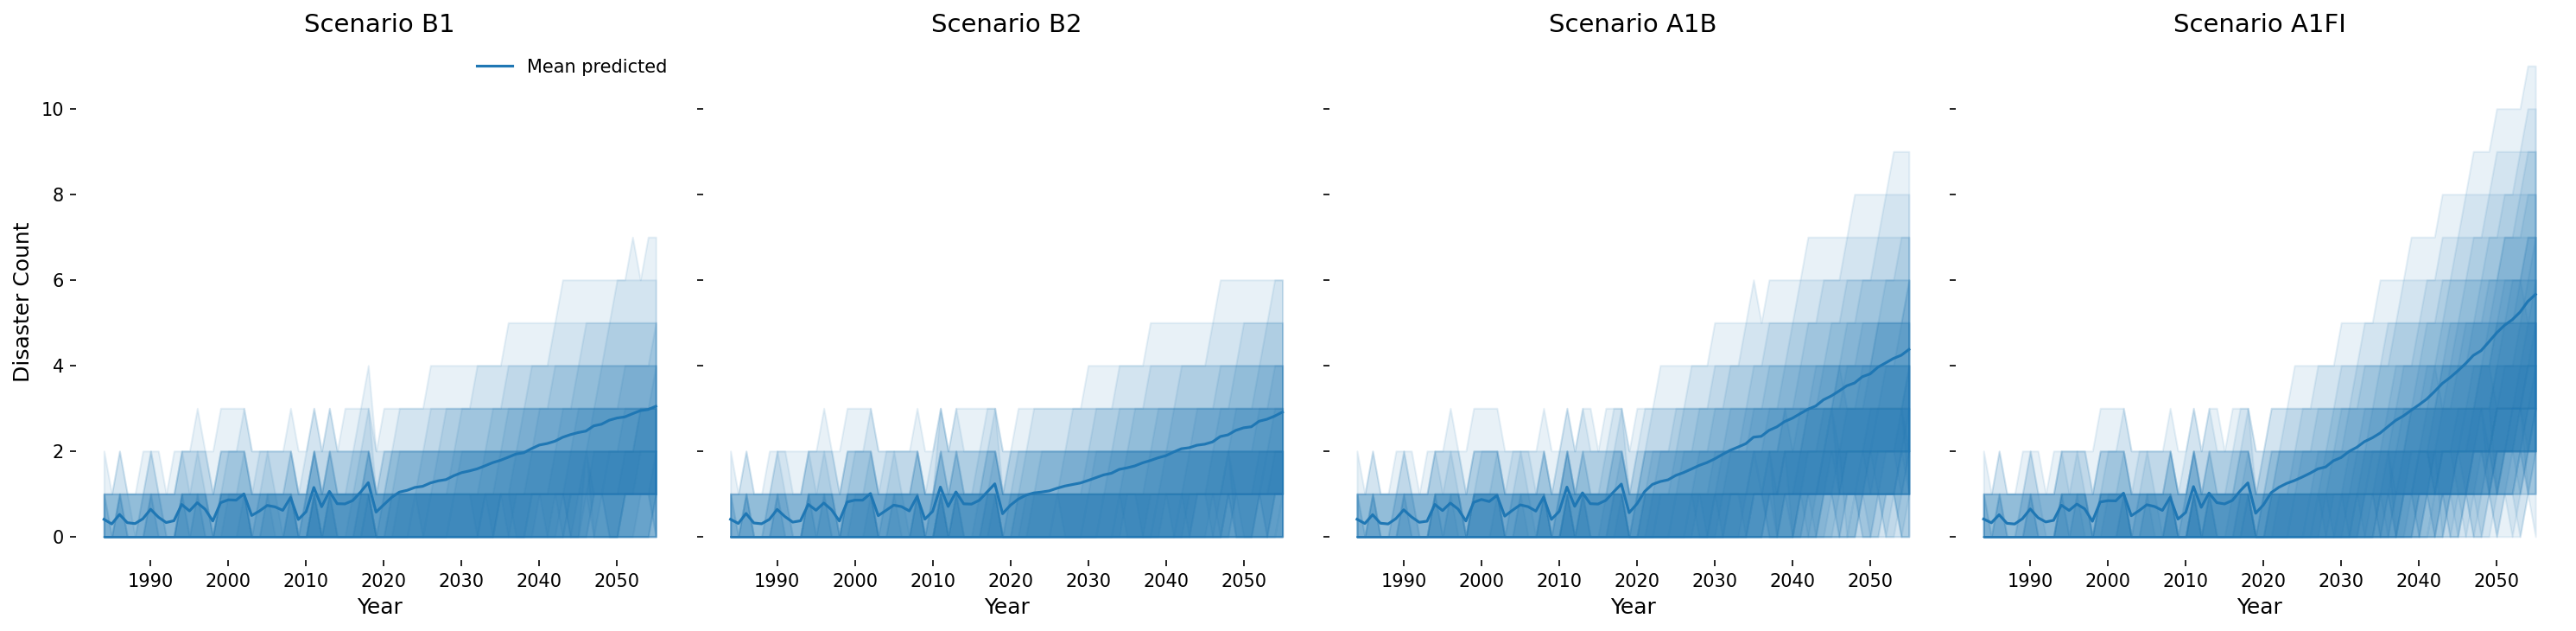
\includegraphics[width=1.15\textwidth]{../notebooks/policy_note/figures/frequency_projections_scenarios.png}}
  \caption{Predicted yearly disaster count for Lao PDR under five IPCC SSP scenarios. Shaded regions indicate the 95\% high density interval. Higher CO\textsubscript{2} scenarios produce accelerating disaster counts, while the most optimistic pathways show a flattening and eventual decline in frequency.}
  \label{fig:freq_scenarios}
\end{figure}

In the near term (2025--2030), all five scenarios produce similar disaster counts because the CO\textsubscript{2} trajectories have not yet diverged substantially. However, by the 2040s and 2050s, the scenarios fan out dramatically. Under SSP5-85 and SSP3-70, the compounding effect of higher atmospheric CO\textsubscript{2} concentrations and warmer ocean temperatures becomes increasingly pronounced, leading to a steep upward trajectory. Under SSP1-19, the opposite occurs: as CO\textsubscript{2} concentrations stabilize and begin to decline (net-zero around 2050, net-negative thereafter), the climate covariates that drive disaster frequency---particularly ocean temperature---respond accordingly, producing a deceleration and eventual reversal of the disaster trend. This non-linear divergence underscores the urgency of early emission reductions: the window in which mitigation can meaningfully alter the trajectory narrows with each decade of delay.

The damage projections in Figure~\ref{fig:dmg_scenarios} show a similar pattern: while the median damage remains moderate across scenarios, the upper tails of the distribution---representing extreme events---diverge substantially. Under SSP5-85, the probability of experiencing very high-damage events grows significantly relative to SSP1-19. Conversely, under SSP1-19, the damage distribution tails stabilize and begin to contract after the mid-2040s. This is precisely where the Bayesian approach adds the most value: by estimating the full probability distribution rather than just the mean, the model reveals that the most policy-relevant differences between scenarios lie in the tails of the damage distribution---the region where traditional point-estimate approaches provide the least information.

\begin{figure}[H]
  \centering
  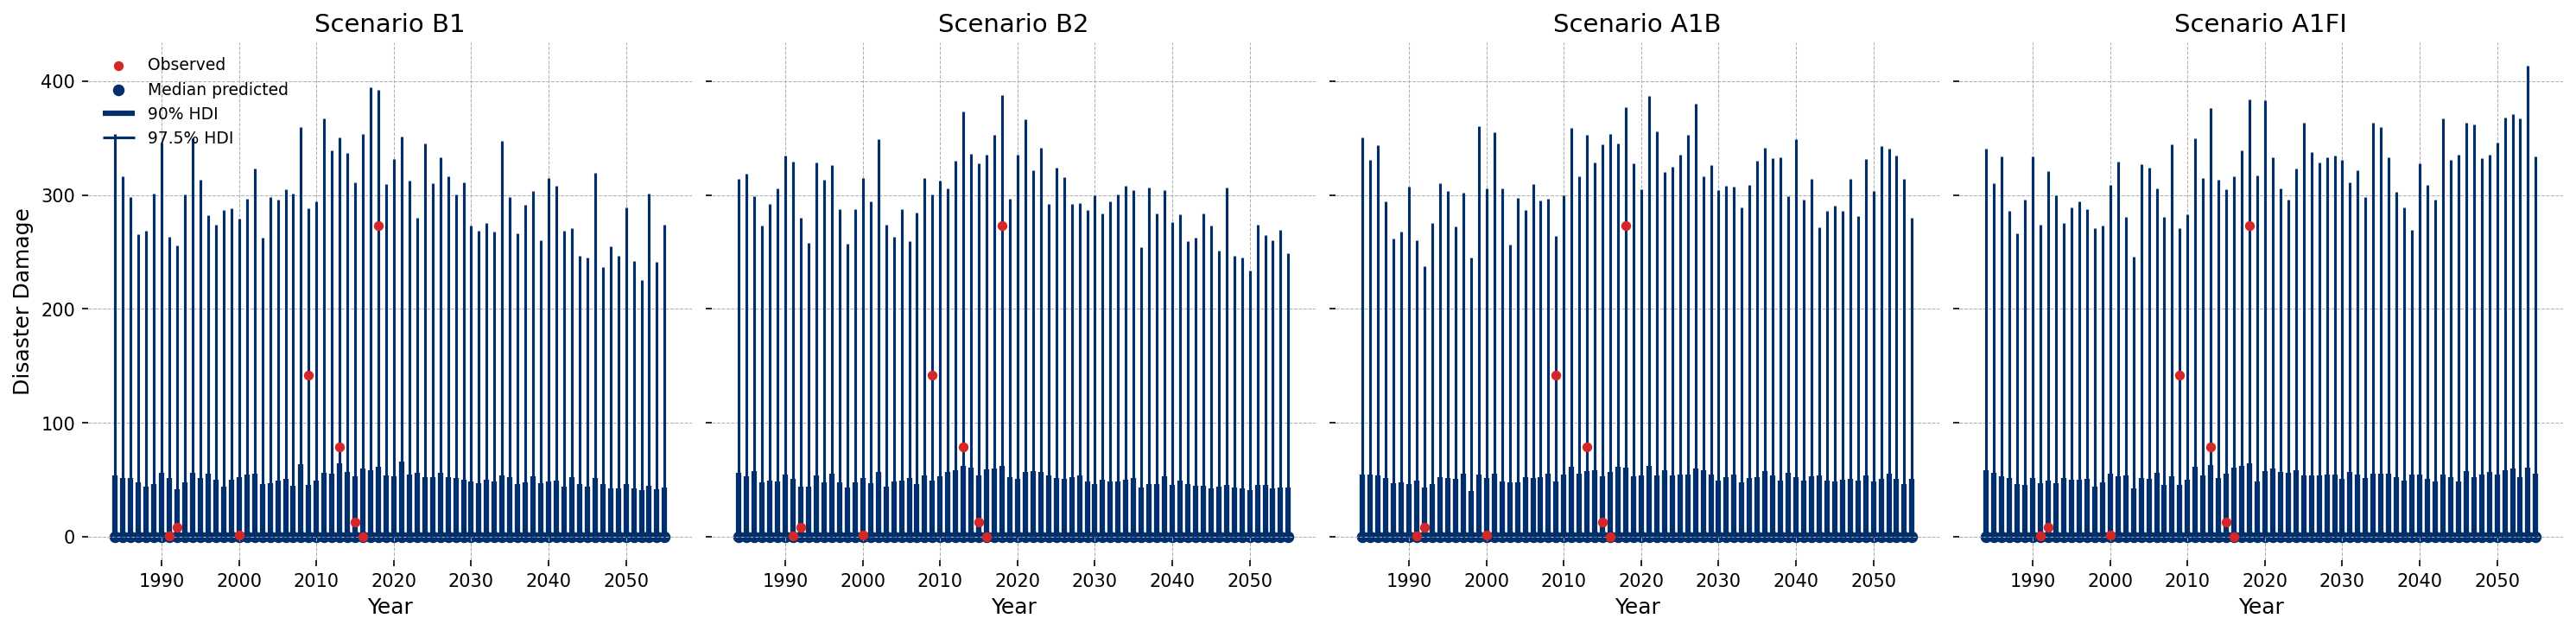
\includegraphics[width=\textwidth]{../notebooks/policy_note/figures/damage_projections_scenarios.png}
  \caption{Predicted disaster damages for Lao PDR under five IPCC SSP scenarios. Thinner segments correspond to the 80\% probability intervals, thicker segments to the 50\% intervals. Under high-emission scenarios the damage tails grow substantially, while the most optimistic pathways show stabilization and contraction of extreme damages.}
  \label{fig:dmg_scenarios}
\end{figure}

\subsection{Impact on Return-Year Damages}

The differences between scenarios become most pronounced for extreme events---precisely the region of the damage distribution that matters most for policy planning, where the Bayesian framework's ability to estimate full posterior distributions adds the greatest value over point-estimate approaches. Figures~\ref{fig:ry10},~\ref{fig:ry50}, and~\ref{fig:ry100} compare the estimated damages at the 10-year, 50-year, and 100-year return periods across scenarios and future decades.

\begin{figure}[H]
  \centering
  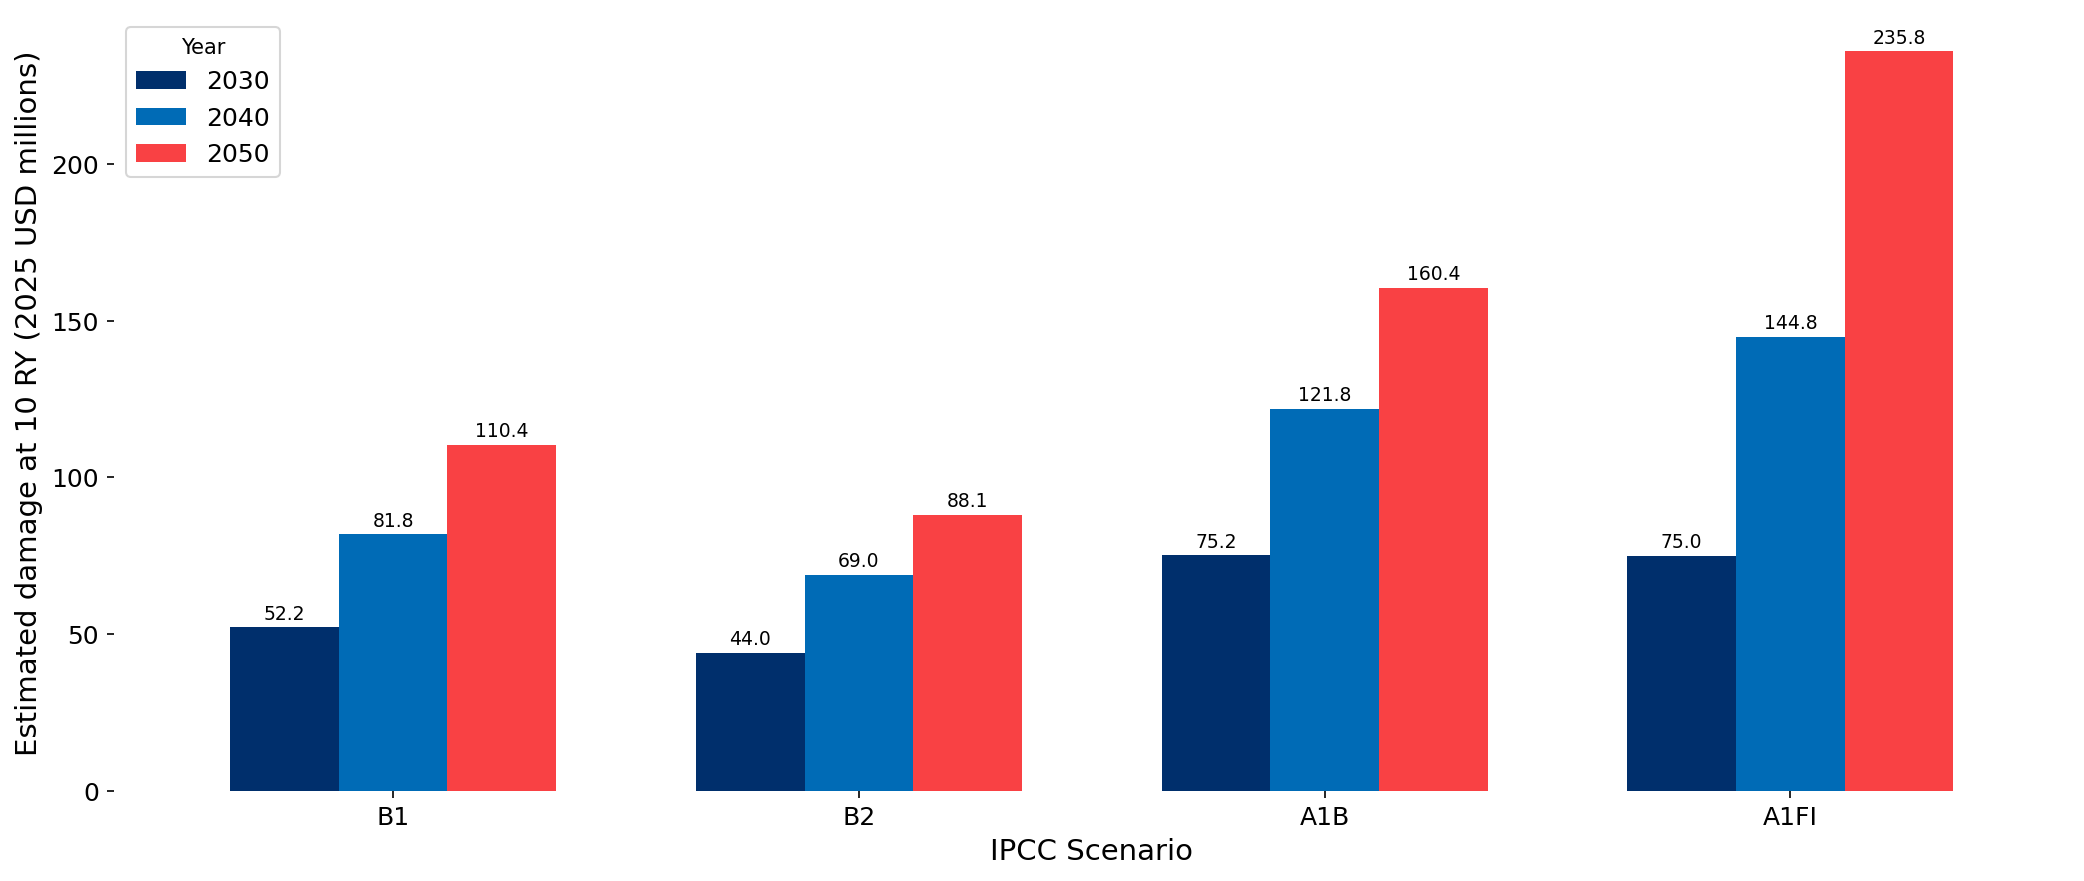
\includegraphics[width=\textwidth]{../notebooks/policy_note/figures/return_year_comparison_scenarios_10_ry.png}
  \caption{Estimated 10-year return period damages (USD millions) under five IPCC SSP scenarios for 2030, 2045, and 2055. Even for relatively frequent events, the gap between low and high emission scenarios is substantial.}
  \label{fig:ry10}
\end{figure}

\begin{figure}[H]
  \centering
  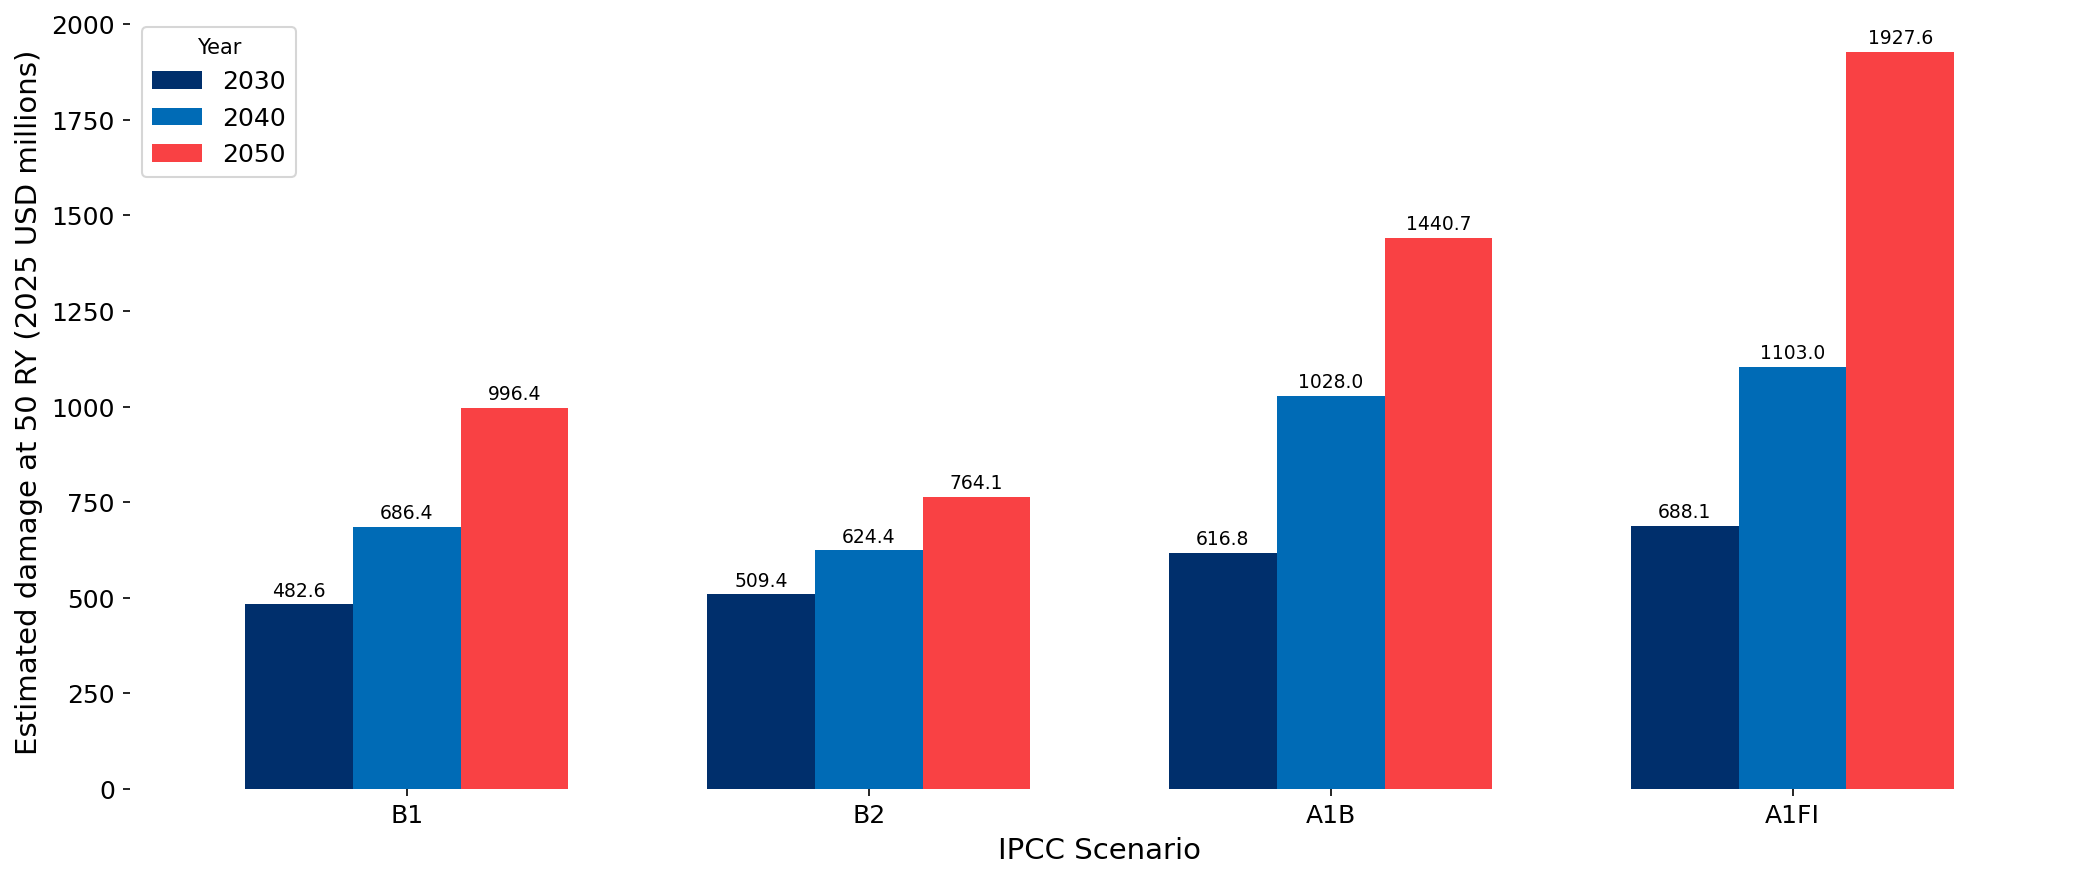
\includegraphics[width=\textwidth]{../notebooks/policy_note/figures/return_year_comparison_scenarios_50_ry.png}
  \caption{Estimated 50-year return period damages (USD millions) under five IPCC SSP scenarios for 2030, 2045, and 2055. The gap between low and high emission scenarios widens over time.}
  \label{fig:ry50}
\end{figure}

\begin{figure}[H]
  \centering
  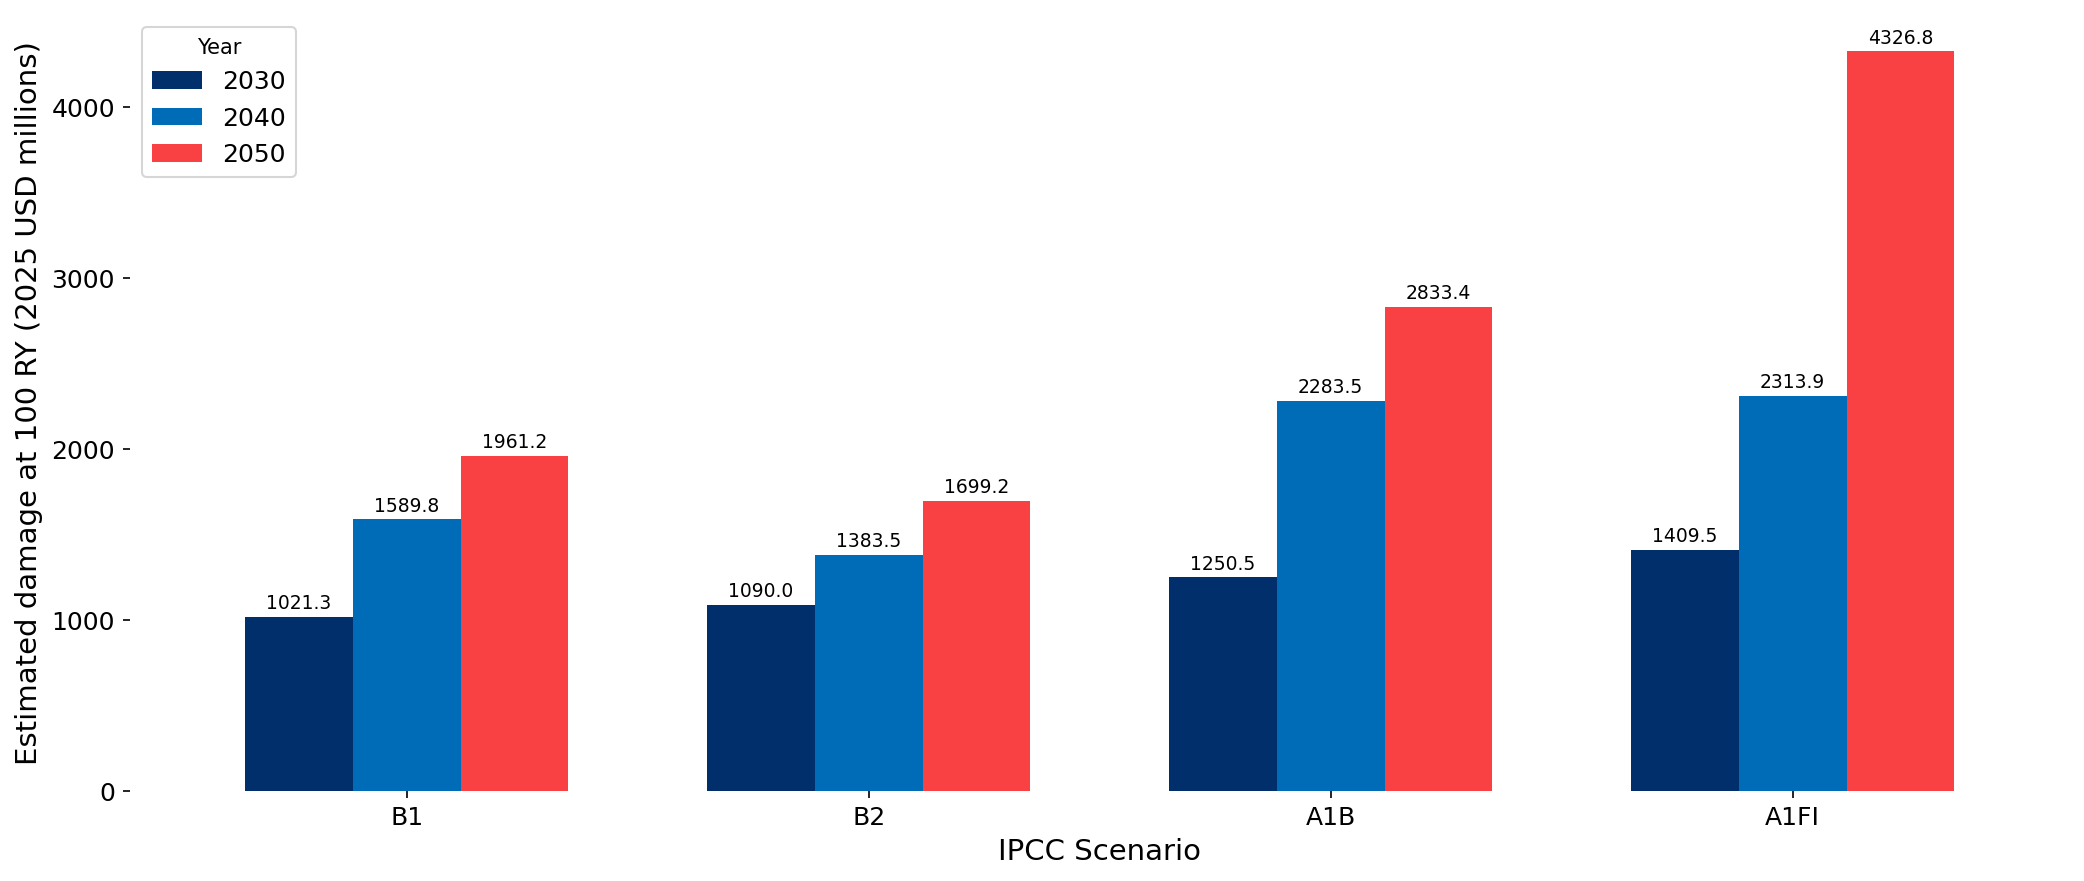
\includegraphics[width=\textwidth]{../notebooks/policy_note/figures/return_year_comparison_scenarios_100_ry.png}
  \caption{Estimated 100-year return period damages (USD millions) under five IPCC SSP scenarios for 2030, 2045, and 2055.}
  \label{fig:ry100}
\end{figure}

Key findings from the scenario comparison:

\begin{itemize}[leftmargin=2em]
  \item \textbf{By 2030}, the 100-year return period damage ranges from \$956 million (SSP1-19) to \$1,222 million (SSP5-85)---a 28\% increase between the most optimistic and most pessimistic emission scenarios. At this early horizon, all five scenarios produce relatively similar results because the CO\textsubscript{2} trajectories have not yet diverged substantially.

  \item \textbf{By 2055}, the gap widens dramatically. The 100-RY damage under SSP5-85 reaches \$4,602 million, while under SSP1-19 it is \$977 million---nearly a five-fold difference. For the 50-RY event, the pattern is similar: \$2,477M (SSP5-85) vs.\ \$456M (SSP1-19).

  \item \textbf{Under SSP1-19, damages actually decrease between 2045 and 2055.} This is the most striking finding: the 100-RY damage declines from \$981M to \$977M, the 50-RY from \$515M to \$456M, and the 10-RY from \$58M to \$50M. This means that aggressive mitigation does not merely slow the increase in disaster risk---it can reverse the trend entirely. The declining slope reflects the physical response of the climate system to stabilizing and then declining CO\textsubscript{2} concentrations under this pathway, which translates into reduced ocean warming and, consequently, lower disaster frequency and severity.

  \item \textbf{The 10-year return period}---representing events that occur roughly once per decade---shows that emission scenarios matter not only for catastrophic tail events but also for recurrent disasters. By 2055, the 10-RY damage under SSP5-85 (\$263M) is more than five times higher than under SSP1-19 (\$50M). These are the events that repeatedly strain government budgets and recovery capacity, and the scenario divergence indicates that higher emissions will substantially increase the recurring fiscal burden of climate-related disasters.

  \item Even the \textbf{moderate scenarios} (SSP1-26, SSP2-45, SSP3-70) produce meaningfully different damages, indicating that each increment of emission reduction yields measurable benefits. SSP1-26 shows a deceleration in damage growth (though not a full reversal as in SSP1-19), while SSP2-45 (\$2,116M at 100-RY by 2055) is already more than double the SSP1-19 level.
\end{itemize}

To place the 2055 results in perspective, the USD~3.6 billion gap between SSP1-19 and SSP5-85 at the 100-year return period represents approximately 18\% of Lao PDR's current GDP. This means that the choice between global emission pathways---a decision largely outside Lao's control---could determine whether a catastrophic disaster event is manageable or economically devastating. The fact that the most optimistic pathway can actually bend the damage curve downward reinforces the importance of pursuing the most ambitious feasible reductions: every increment of avoided CO\textsubscript{2} translates into measurably lower disaster risk for vulnerable countries like Lao PDR.

These results reveal a fundamental asymmetry: Lao PDR contributes negligibly to global CO\textsubscript{2} emissions---less than 0.1\% of the global total---yet bears disproportionate consequences from higher-emission pathways chosen by major emitters. The USD~3.6 billion gap between SSP1-19 and SSP5-85 quantifies what might be called the \textit{adaptation premium}: the additional cost that vulnerable countries must bear, or insure against, when the world follows a high-emission trajectory rather than an ambitious mitigation pathway. Conversely, the declining damage trajectory under SSP1-19 demonstrates that ambitious global action can deliver tangible benefits to the most vulnerable: not just a slower deterioration, but an actual improvement in disaster risk outcomes. This dual finding strengthens the case for international climate finance mechanisms that channel both mitigation support and adaptation assistance to countries whose risk exposure is shaped by decisions largely beyond their control. While Lao PDR cannot meaningfully influence global emission trajectories, it can invest in local adaptation infrastructure to reduce the impact of the disasters that do occur. The following section evaluates one such intervention.

% =============================================================================
% 5. RESULTS: FLOOD WALL SIMULATIONS
% =============================================================================
\section{Results: Flood Wall Simulations}

\subsection{City Selection and Baseline Risk}

We focus on three population centers located near high-risk areas: Attapeu, Vientiane, and Pakse. Figure~\ref{fig:lao_map} shows their locations on the geospatial risk heatmap, where lighter colors indicate higher disaster probability. These cities were selected to represent different risk profiles: Attapeu lies in a river-dominated risk zone in the southeast, Vientiane is the capital and largest population center with a complex multi-factor risk profile, and Pakse is a medium-sized city in the south with moderate baseline risk.

\begin{figure}[H]
  \centering
  
\includegraphics[width=0.5\textwidth]{images/loc_lao_map.png}
  \caption{Geospatial risk map of Lao PDR with the three cities selected for flood wall simulations. The heatmap represents the normalized probability of disaster occurrence at each grid point.}
  \label{fig:lao_map}
\end{figure}

\subsection{Damage Reduction Results}

Figure~\ref{fig:wall_bars} presents the estimated damages at different return periods for each city under the three scenarios (no wall, intermediate wall, full wall). Table~\ref{tab:wall_reduction} summarizes the damage reduction in absolute terms.

\begin{figure}[H]
  \centering
  
\includegraphics[width=\textwidth]{images/flood_wall_bar_chart_all_cities.png}
  \caption{Estimated damages (USD millions) at 25, 30, 40, and 50-year return periods for Attapeu, Pakse, and Vientiane under three scenarios: no wall (baseline), intermediate wall (median river distance), and full wall (maximum river distance). Year 2030 projections.}
  \label{fig:wall_bars}
\end{figure}

\begin{table}[H]
  \centering
  \caption{Damage reduction from flood wall interventions (USD millions), year 2030. Values represent the decrease in expected damages relative to the no-wall baseline.}
  \label{tab:wall_reduction}
  \small
  \begin{tabular}{llrr}
    \toprule
    \textbf{City} & \textbf{Return Period} & \textbf{Full Wall} & \textbf{Intermediate Wall} \\
    \midrule
    \multirow{4}{*}{Attapeu}   & 25 RY & 13.79 &  9.72 \\
                               & 30 RY & 17.34 & 11.90 \\
                               & 40 RY & 26.22 & 19.07 \\
                               & 50 RY & 35.91 & 26.38 \\
    \midrule
    \multirow{4}{*}{Pakse}     & 25 RY &  0.19 &  0.50 \\
                               & 30 RY &  0.51 &  0.58 \\
                               & 40 RY &  0.18 &  0.14 \\
                               & 50 RY &  1.32 &  1.45 \\
    \midrule
    \multirow{4}{*}{Vientiane} & 25 RY &  0.47 &  0.25 \\
                               & 30 RY &  0.46 &  0.22 \\
                               & 40 RY &  0.76 &  0.62 \\
                               & 50 RY &  0.68 &  0.30 \\
    \bottomrule
  \end{tabular}
\end{table}

The results reveal sharply different effectiveness across cities:

\begin{itemize}[leftmargin=2em]
  \item \textbf{Attapeu} shows the largest benefit. A full wall reduces 50-RY damages by \$35.9 million (73\% reduction), and even an intermediate wall achieves a \$26.4 million reduction (54\%). This is because Attapeu's risk profile is dominated by river proximity: the geospatial model's HSGP component and the distance-to-river covariate both contribute strongly to the local risk at this location. When the effective distance to the river is increased, the model predicts a dramatic reduction in event probability, which propagates through the damage curve to produce large absolute savings. The scaling of the benefit with return period---from \$13.8M at 25-RY to \$35.9M at 50-RY---reflects the fact that flood walls are most valuable precisely when they are needed most: during the rarer, more extreme events that cause the greatest damage.

  \item \textbf{Pakse} shows minimal benefit (5--6\% reduction at 50 RY). Despite being located near rivers, Pakse's overall risk profile is relatively low, and the river distance component contributes less to its total risk compared to Attapeu. The HSGP spatial component assigns Pakse a lower baseline probability, which limits the absolute damage savings achievable through river-based interventions. The small and inconsistent reductions across return periods suggest that other risk factors---not addressable by a flood wall---dominate Pakse's exposure.

  \item \textbf{Vientiane} shows moderate but limited benefit (13\% reduction at 50 RY with a full wall). As the capital and largest urban center, Vientiane's risk is driven more by regional disaster patterns captured by the Gaussian Process component---reflecting the broader clustering of disasters around major population centers, high population density, and economic concentration---than by river proximity alone. A flood wall addresses only one component of a multi-factor risk profile. For Vientiane, complementary strategies such as urban drainage improvements, early warning systems, and land-use planning would likely yield greater marginal returns than river-based infrastructure alone.
\end{itemize}

This analysis demonstrates that flood wall effectiveness depends critically on the local risk decomposition. Cities where river proximity is the dominant risk factor---as identified by the geospatial model's component analysis---benefit most from river-based interventions. In contrast, cities where regional patterns, coastal exposure, or other factors dominate require a broader set of adaptation strategies.

These results provide a first overview of the potential benefits of flood wall interventions, and should be complemented by detailed engineering analysis before investment decisions are made. Nevertheless, the geospatial risk decomposition offers a valuable screening tool for policymakers: it identifies which cities are most likely to benefit from river-based infrastructure, helping to prioritize where in-depth hydrological and engineering assessments should be conducted. Without this kind of preliminary risk decomposition, a one-size-fits-all approach to flood defense could waste resources in cities where the dominant risk factors are not addressable by flood walls, while missing opportunities for high-impact interventions in cities like Attapeu.

The methodology demonstrated here is scalable to other types of infrastructure interventions. Just as flood walls are simulated by modifying the distance-to-river covariate, other interventions---such as improved drainage systems, levees, or coastal defenses---could be evaluated by adjusting the relevant geospatial covariates in the model. This flexibility makes the PGR framework a general-purpose tool for evaluating adaptation infrastructure, not just flood walls.

From a cost-benefit perspective, the damage reductions quantified above provide the ``benefit'' side of an investment analysis. For instance, the USD~35.9 million reduction in 50-year return period damages for Attapeu under a full wall scenario can be directly compared against the construction and maintenance costs of a flood wall to assess investment feasibility. While engineering cost estimates are outside the scope of this analysis, the probabilistic damage curves provide exactly the inputs needed for such an evaluation. Moreover, combining the flood wall analysis with the CO\textsubscript{2} scenario results from the previous section would reveal how infrastructure requirements scale under different emission pathways: higher-emission scenarios, which produce larger expected damages, would correspondingly increase the economic returns from flood protection---but may also require more robust and costly defenses to achieve the same level of protection.

% =============================================================================
% 6. CONCLUSIONS
% =============================================================================
\section{Conclusions}

This policy note demonstrates the PGR model's capacity to inform climate adaptation policy in Lao PDR through baseline projections, scenario analysis, and local intervention simulations. For the full methodological details, including model specifications, estimation procedures, and diagnostic results, the reader is referred to the companion paper \cite{saldarriaga2026}.

\textbf{Baseline projections reveal escalating risk.} Even under current trends, the model projects that disaster frequency will approximately triple by 2060, and 100-year return period damages will rise from USD~611 million in 2000 to over USD~2.1 billion by 2055. Critically, moderate-frequency events (10-year return periods) also show a five-fold increase, implying that recurring disaster costs will grow substantially alongside catastrophic tail risks. The geospatial model further identifies specific high-risk zones---particularly river confluence areas---where this escalation will be most acute.

\textbf{Global emission pathways matter for local risk---and ambitious mitigation can reverse the trend.} The CO\textsubscript{2} scenario analysis---using five IPCC SSP pathways with conditionally adjusted climate covariates---shows that higher emission trajectories translate directly into greater disaster risk for Lao PDR. By 2055, the 100-year return period damage under SSP5-85 (\$4,602M) is nearly five times higher than under SSP1-19 (\$977M), a gap of USD~3.6 billion representing approximately 18\% of Lao PDR's current GDP. Critically, under SSP1-19, disaster damages actually decrease between 2045 and 2055 across all return periods, meaning that the most ambitious mitigation pathway does not merely slow the deterioration but reverses it. This finding provides a concrete, quantifiable demonstration that early and aggressive emission reductions can deliver real improvements in disaster risk for vulnerable countries.

\textbf{Local interventions can be highly effective---but must be targeted.} The flood wall simulations show that infrastructure investments can achieve dramatic damage reductions in cities where river proximity is the primary risk driver. In Attapeu, a full flood wall could reduce 50-year return period damages by 73\%. However, the same intervention yields minimal benefit in cities like Pakse and Vientiane, where other risk factors dominate. This highlights the importance of using geospatial risk decomposition to prioritize and design infrastructure investments.

\textbf{Policy recommendations:}
\begin{itemize}[leftmargin=2em]
  \item Prioritize flood defense infrastructure in cities where the geospatial model identifies river proximity as the dominant risk factor.
  \item Develop complementary adaptation strategies for cities where regional disaster patterns drive risk, such as early warning systems and land-use planning.
  \item Advocate for alignment with low-emission global CO\textsubscript{2} pathways, as even moderate reductions in global emissions yield measurable benefits for Lao PDR's disaster exposure.
  \item Use the probabilistic framework to evaluate additional intervention scenarios, such as combined flood walls and drainage improvements, or alternative city selections.
\end{itemize}

The PGR model's scenario-based framework provides a flexible tool for evaluating policy interventions before implementation, enabling evidence-based prioritization of climate adaptation investments.

\textbf{Broader implications.} Although this analysis focuses on Lao PDR, the PGR methodology is not country-specific. The framework can be applied to any country with historical disaster records, and the hierarchical Bayesian structure is particularly well-suited to data-scarce developing countries, where it borrows strength across countries to improve local estimates. The methodology can also be extended to other hazard types---including droughts, wildfires, and extreme temperature events---by adjusting the disaster classification and relevant covariates. Furthermore, the probabilistic outputs---damage curves expressed in monetary terms at specific return periods---are directly compatible with standard cost-benefit analysis frameworks, enabling development finance institutions to compare expected avoided damages against intervention costs.

\textbf{Limitations and future work.} Several limitations should be noted. The model relies on historical disaster records from EM-DAT \cite{emdat2024}, which may undercount events in earlier decades and in remote areas, potentially leading to underestimation of baseline risk. The flood wall simulation modifies the distance-to-river covariate rather than explicitly modeling engineering infrastructure; future work could integrate hydraulic models to more precisely estimate protective capacity The time series projections assume continuation of historical trends and do not capture structural breaks such as rapid industrialization or major policy shifts. Key extensions that would strengthen the framework include: integrating adaptation cost estimates for full cost-benefit analysis, extending to additional Mekong region countries, and incorporating compound disaster risks---where one event triggers or amplifies subsequent events---which are expected to become more prevalent under climate change \cite{ipcc2023ar6}.


\textbf{A call to action.} The results presented in this note underscore the urgency of proactive climate adaptation in Lao PDR. The non-linear divergence between emission scenarios means that the window for effective action narrows with each year of delay: under high-emission pathways, disaster risk accelerates sharply, while the most ambitious mitigation pathways can actually bend the curve downward---but only if action is taken early enough for the climate system to respond. Early investments in both local infrastructure and international emission reductions yield disproportionately large benefits compared to equivalent investments made later. The PGR model provides the quantitative evidence base needed to design, prioritize, and evaluate such investments---contributing to a shift from reactive disaster response toward proactive, evidence-based climate adaptation planning for developing countries.

% =============================================================================
% REFERENCES
% =============================================================================
\makeatletter
\renewcommand{\@biblabel}[1]{}
\makeatother
\begin{thebibliography}{99}

\bibitem{abril2023pymc}
Abril-Pla, O., Andreani, V., Carroll, C., Dong, L., Fonnesbeck, C. J., Kochurov, M., Kumar, R., Lao, J., Luhmann, C. C., Martin, O. A., Osthege, M., Vieira, R., Wiecki, T., and Zinkov, R. (2023).
``PyMC: A Modern, and Comprehensive Probabilistic Programming Framework in Python.''
\textit{PeerJ Computer Science}, 9, e1516.

\bibitem{besag1991}
Besag, J., York, J., and Molli\'{e}, A. (1991).
``Bayesian Image Restoration, with Two Applications in Spatial Statistics.''
\textit{Annals of the Institute of Statistical Mathematics}, 43(1), 1--20.

\bibitem{cavallo2011}
Cavallo, E. and Noy, I. (2011).
``Natural Disasters and the Economy---A Survey.''
\textit{International Review of Environmental and Resource Economics}, 5(1), 63--102.

\bibitem{emdat2024}
CRED (2024).
\textit{EM-DAT: The International Disaster Database}.
Centre for Research on the Epidemiology of Disasters, Universit\'{e} catholique de Louvain, Brussels, Belgium.

\bibitem{laopdr_pdna2018}
Government of Lao PDR (2018).
\textit{Post-Disaster Needs Assessment: 2018 Floods, Lao PDR}.
United Nations Lao PDR.

\bibitem{howard2017}
Howard, P. H. and Sterner, T. (2017).
``Few and Not So Far Between: A Meta-analysis of Climate Damage Estimates.''
\textit{Environmental and Resource Economics}, 68(1), 197--225.

\bibitem{ipcc2000sres}
IPCC (2000).
\textit{Special Report on Emissions Scenarios}.
Cambridge University Press.

\bibitem{ipcc2021ar6wg1}
IPCC (2021).
\textit{Climate Change 2021: The Physical Science Basis. Contribution of Working Group I to the Sixth Assessment Report}.
Cambridge University Press.

\bibitem{ipcc2022ar6wg2}
IPCC (2022).
\textit{Climate Change 2022: Impacts, Adaptation and Vulnerability. Contribution of Working Group II to the Sixth Assessment Report}.
Cambridge University Press.

\bibitem{ipcc2023ar6}
IPCC (2023).
\textit{Climate Change 2023: Synthesis Report. Contribution of Working Groups I, II and III to the Sixth Assessment Report}.
Geneva, Switzerland.

\bibitem{lehner2013}
Lehner, B. and Grill, G. (2013).
``Global River Hydrography and Network Routing: Baseline Data and New Approaches to Study the World's Large River Systems.''
\textit{Hydrological Processes}, 27(15), 2171--2186.

\bibitem{lopez2015}
L\'{o}pez, R., Thomas, V., and Troncoso, P. (2015).
``Climate Change and Natural Disasters.''
Working Paper.

\bibitem{nicholls2021rcmip}
Nicholls, Z., Meinshausen, M., Lewis, J., et al. (2021).
Reduced Complexity Model Intercomparison Project Phase 2: Synthesizing Earth system knowledge for probabilistic climate projections.
\textit{Earth's Future}, 9(6), e2020EF001900.
https://doi.org/10.1029/2020EF001900

\bibitem{noaa_co2_2024}
NOAA (2024).
\textit{Trends in Atmospheric Carbon Dioxide}.
National Oceanic and Atmospheric Administration, Global Monitoring Laboratory.

\bibitem{nordhaus2019}
Nordhaus, W. D. (2019).
``Climate Change: The Ultimate Challenge for Economics.''
\textit{American Economic Review}, 109(6), 1991--2014.

\bibitem{openai2024gpt4omini}
OpenAI (2024).
``GPT-4o mini: Advancing Cost-Efficient Intelligence.''
OpenAI Research Blog.

\bibitem{saldarriaga2026}
Saldarriaga, C., Grabowski, J., and Rielaender, J. (2026).
``Estimating Climate Change Risk Exposure: A Probabilistic Approach.''
Working Paper, OECD Development Center.

\bibitem{gpcc_2022}
Schneider, U., Becker, A., Finger, P., Rustemeier, E., and Ziese, M. (2022).
\textit{GPCC Full Data Monthly Product Version 2022}.
Global Precipitation Climatology Centre.

\bibitem{solin2020}
Solin, A. and S\"{a}rkk\"{a}, S. (2020).
``Hilbert Space Methods for Reduced-Rank Gaussian Process Regression.''
\textit{Statistics and Computing}, 30(2), 419--446.

\bibitem{vanaalst2006}
Van Aalst, M. K. (2006).
``The Impacts of Climate Change on the Risk of Natural Disasters.''
\textit{Disasters}, 30(1), 5--18.

\bibitem{worldbank_wdi_2024}
World Bank (2024).
\textit{World Development Indicators}.
Washington, DC: The World Bank.

\bibitem{zhang_noaa_2019}
Zhang, H.-M., Huang, B., Lawrimore, J., Menne, M., and Smith, T. (2019).
\textit{NOAA Global Surface Temperature Dataset (NOAAGlobalTemp)}.
National Centers for Environmental Information.

\end{thebibliography}

\end{document}
